\chapter{Vergleich weiterer Aspekte}


\section{Arithmetische Überläufe}
\label{sec:implementation:overflows}

in frama-c stellen gut erkennbar

in VeriFast lemma limits

 Im Werkzeug VeriFast
ist es eine Option, die für die Verifizierung an - oder ausgeschaltet werden kann. In Frama-C ... \todo{testen}

\section{Aliasing}

copy oder move zeigen und unterschied zwischen acsl und verifast

memmove kontrakt

\lstinline{\seperated}



\section{Arbeit mit den Werkzeugen}
\todo{section ggf. in anderes kapitel auslagern und überarbeiten}
Im Gegensatz zu VeriFast bezeichnet ACSL nicht ein vollständiges Werkzeug, sondern ausschließlich
die Annotationssprache. Die Verarbeitung übernimmt eine Kombination aus Frama-C, Why\footnote{
\url{http://why.lri.fr/}} und daran angeschlossene Beweiser wie Alt-Ergo\footnote{\url{http://alt-ergo.lri.fr/}}
oder Z3\footnote{\url{http://research.microsoft.com/en-us/um/redmond/projects/z3/}}. Das ermöglicht 
eine voneinander unabhängige Weiterentwicklung der Sprache und des Verifizierungs-Backends. Beispielsweise 
können für spezielle Probleme somit auch spezialisierte Beweiser eingesetzt werden. Im Extremfall kann
dann die Verifizierung einer Implementierung nicht durch einen, sondern nur durch die Summe aller
Beweiser gelingen.

\begin{figure}[H]
	\centering
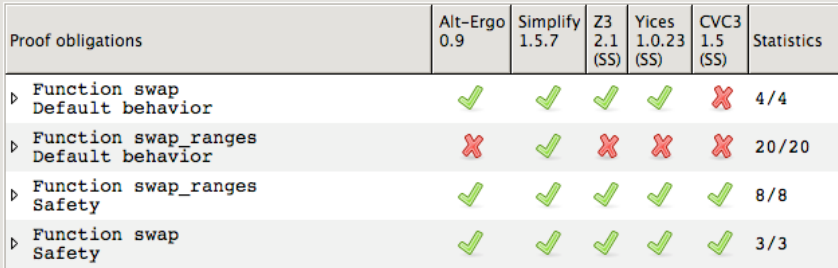
\includegraphics[width=1.0\textwidth]{images/why-multiple-provers.png}
\caption{Verifizierung mit mehreren Beweisern auf der Why-Plattform}
\end{figure}

In VeriFast hingegen sind die Sprache und die Verifizierung in einer Software zusammen gefasst,
es ist nicht möglich den integrierten Z3 Beweiser auszutauschen. Dafür ermöglicht VeriFast das
einfacherere Nachvollziehen der Verifizierung direkt im Quellcode. Insbesondere die Möglichkeit
Haltepunkte zu setzen, erleichtert die Arbeit enorm, da der Zustand der symbolischen Ausführung
inspizierbar ist und schnell erkennen lässt an welcher Stelle es noch hakt.

Mit ACSL ist so etwas nicht denkbar, da die Verifizierung auf einem anderem Prinzip beruht. Die
in Why gezeigten \todo{screenshot einfügen?}Ausgaben der Formeln sind zwar hilfreich, aber längst nicht so einfach nachvollziehbar und
verständlich wie der Zustand in VeriFast.

Für beide Werkzeuge aber gilt, dass sie leider nur alleine lauffähig sind und nicht im Rahmen
einer Entwicklungsumgebung wie Eclipse\footnote{\url{www.eclipse.org}} genutzt werden können. 
Für die Verifizierung muss also der Arbeitsfluss unterbrochen werden. Denn auch wenn die Verifizierung
nicht vom Entwickler durchgeführt werden sollte, wäre es hilfreich in einer einzigen integrierten Umgebung
den Code auszuführen, zu testen, zu debuggen und verifizieren zu können.

Mindestens genauso wichtig aber ist die Unterstützung für die Kommandozeile, die beide Werkzeuge
mitbringen. Damit ist die Verifizierung auch automatisiert möglich und die Einbettung in eine
Continous Integration\footnote{\url{http://de.wikipedia.org/wiki/Kontinuierliche_Integration}}-Umgebung möglich.

Ein wichtiger Unterschied der beiden Untersuchungsobjekte ist die unterschiedliche Verifizierungs-Geschwindigkeit
in der Praxis. Denn VeriFast ist um ein Vielfaches schneller\cite[Kap. 3]{jac10-1} als Frama-C. 

Daraus lässt sich jedoch keine Schlussfolgerung bzgl. der Qualität der Werkzeuge ziehen. Das unterschiedliche Tempo ist 
vielmehr ein Resultat der unterschiedlichen Ansätze: VeriFast erwartet mehr Einsatz von der verifizierenden Person, da
die logischen Folgerungen des Werkzeugs eher klein sind und darum viele Annotationen in der Implementierung nötig sind.
Frama-C hingegen kann auch komplexere Berechnungen ausführen, kommt mit weniger Annotationen aus, ist daher aber auch
wesentlich langsamer.

- frama c gui lässt kein bearbeiten des codes zu

